\documentclass{article}
\usepackage{graphicx} % Required for inserting images
\usepackage{amsmath}
\usepackage{amssymb}

\title{Homework 3}
\author{Ameyassh Nagarajan}
\date{May 2024}

\begin{document}

\maketitle

\section{Question 1}
\textbf{Prove that the following problem is coNP-complete:}

\[
\text{EQV} = \{(\phi_1,\phi_2) \mid \phi_1 \text{and} \phi_2 \text{ are logically equivalent boolean formulas} \}
\]

\subsubsection*{EQV is in coNP}
The problem EQV is defined as determining whether two Boolean formulas, $\phi_1$ and $\phi_2$, are logically equivalent, meaning they produce the same results for all variable assignments. A problem is in coNP if the complement of the problem can be verified in polynomial time.

\subsubsection*{Complement of EQV}
The complement of EQV involves pairs of Boolean formulas $(\phi_1, \phi_2)$ that are not equivalent. To verify non-equivalence, one needs to find an assignment of the variables where the evaluations of $\phi_1$ and $\phi_2$ differ.

\subsubsection*{Verification Process}
\begin{enumerate}
    \item Guess an assignment of the variables.
    \item Evaluate both $\phi_1$ and $\phi_2$ under this assignment.
    \item Check if the outputs differ.
\end{enumerate}
This process can be executed in polynomial time, confirming that the non-equivalence can be verified efficiently, thereby placing EQV in coNP.

\subsection*{Definitions}
\subsubsection*{Tautology (TAUT)}
The Tautology problem involves determining whether a Boolean formula, denoted $\phi$, evaluates to true for every possible assignment of its variables.

\subsubsection*{Equivalence (EQV)}
The Equivalence problem requires establishing whether two Boolean formulas, $\phi_1$ and $\phi_2$, are logically equivalent. Two formulas are considered equivalent if they yield the same truth value under every possible assignment of their variables. Moreover, for the purpose of this proof, both formulas must share the exact same set of variables.

\subsection*{Reduction from TAUT to EQV}

\subsubsection*{Idea for the reduction}
The main idea for the reduction is to convert to a TAUT to an EQV problem. To
show that, solving EQV is atleast as hard as TAUT, which is a well known
coNP-complete problem.

\subsubsection*{Constructing the Equivalence Test}
To perform this reduction, we employ the following steps:
\begin{itemize}
  \item Let $\phi_1 = \phi$, where $\phi$ is the formula to be tested for tautology.
  \item Construct $\phi_2$ to be explicitly tautological and include all variables present in $\phi_1$. This ensures that both formulas share the same variable set. For simplicity and to maintain generality, let:
    \[
    \phi_2 = \bigwedge_{i=1}^{n} (x_i \lor \lnot x_i),
    \]
    where $x_i$ are the variables in $\phi$. This construction guarantees that $\phi_2$ is tautologically true.
\end{itemize}

\subsubsection*{Logical Implication of the Reduction}
By constructing $\phi_1$ and $\phi_2$ as above, the equivalence $\phi_1 \equiv \phi_2$ serves as a direct test for the tautological nature of $\phi_1$. Specifically:
\begin{itemize}
  \item If $\phi_1 \equiv \phi_2$, then $\phi_1$ must evaluate to true under all variable assignments, just like $\phi_2$, confirming that $\phi_1$ is a tautology.
  \item Conversely, if $\phi_1$ is not a tautology, there exists at least one assignment under which $\phi_1$ evaluates to false, thereby breaking its equivalence to the always true $\phi_2$.
\end{itemize}

\pagebreak
\subsubsection*{Polynomial Time Reduction}

The reduction from the Tautology problem (TAUT) to the Equivalence problem (EQV) takes polynomial time, proving that it is a valid Karp reduction. The process involves:

\begin{itemize}
    \item \textbf{Copying the TAUT Formula:} Directly replicating the tautology formula, \( \phi \), as \( \phi_1 \). This step is linear with respect to the length of \( \phi \).
    \item \textbf{Constructing \( \phi_2 \):} Formulating \( \phi_2 \) as \( (x_1 \lor \lnot x_1) \land \ldots \land (x_n \lor \lnot x_n) \), which scales linearly with the number of variables, \( n \), in \( \phi_1 \).
\end{itemize}

Both steps ensure the reduction is completed in polynomial time.

\subsection*{Conclusion}
This reduction shows that EQV is at least as hard as TAUT and that solving EQV will yield a result for TAUT this also goes on to show that EQV is coNP-Hard. And since EQV is in coNP and it is coNP-Hard, EQV is coNP-Complete.



\pagebreak
%-----------------------------------------------------------------------%
%QUESTION 2
\section{Question 2}
\textbf{Problem 2:} Show that the following problem is NP-complete: Given a set of linear inequalities over a set of variables \(x_1, \dots, x_n\), determine whether there is an assignment of integers to the \(x_i\)'s that satisfies all inequalities.

\textbf{Example:}
\begin{align*}
    x_1 + 3x_2 - x_5 &\geq 3 \\
    2x_2 - x_4 &\leq x_3 \\
    x_1 + x_2 + x_3 + x_4 + x_5 &\geq 0
\end{align*}

This system of inequalities is satisfied by \(x_1 = 10\), \(x_2 = 3\), \(x_3 = x_4 = -3\), \(x_5 = 0\) (among many others).

\subsubsection*{Defining the Problem}
Let us begin by calling this language as \textbf{INEQ}, it is defined such that:

\[
\text{INEQ} = \left\{ (A, \vec{b}, \vec{c}) \mid \text{There exists } \vec{x} \in \mathbb{Z}^n \text{ such that } A\vec{x} \leq \vec{b} \text{ and } A\vec{x} \geq \vec{c} \right\}
\]

where \( A \) is a matrix of coefficients, \( \vec{b} \) and \( \vec{c} \) are vectors of bounds, and \( \vec{x} \) is a vector of integer variables.



% When given a CNF formula we can interpret it in such a way that each clause evaluates to atleast 1, that is the sum of all the literals in the clause is at least 1 or greater. We can use this information to convert the Clause in a CNF  to a inequality, such that we add up all the literals $x_i$ in a clause and make sure that it is greater than or equal to one. To hande negations, we can just write $1-x_i$. That is if $x_i$ is 1 in the clause then negation of $x_i$ is 0, and this can be implied using the rule that we have imposed in above. Thus if we can reduce each clause in the CNF to an inequality, and check if each inequality evaluates to at least 1. We can convert SAT to INEQ. Therefore showing that INEQ is atleast as hard as SAT. This reduction can be done in polynomial time, that is if given an input CNF formula $\psi$ we can convert it to an inequality in a polynomial number of steps of the input formula, thereby showing that SAT can reduce to INEQ in polyime. 

\subsubsection*{ INEQ is in NP}
To classify a problem as belonging to NP, we need to establish that any proposed solution to the problem can be verified efficiently—specifically, in polynomial time relative to the size of the input. This does not necessarily imply that finding a solution is easy, but that checking a given solution is computationally manageable.

we focus on how to verify a given solution effectively.

\textbf{Verification Steps for INEQ:}
\begin{itemize}
    \item \textbf{Matrix-Vector Multiplication:} Start by computing the product \(A\vec{x}\), where \(A\) is a matrix and \(\vec{x}\) is a vector of integers. This calculation involves a series of multiplications and additions based on the dimensions of \(A\) and \(\vec{x}\), which is typically a polynomial-time operation.
    \item \textbf{Comparison Against Bounds:} Once \(A\vec{x}\) is computed, each component of the resulting vector must be compared against the corresponding components of vectors \(\vec{b}\) and \(\vec{c}\). This step checks if each inequality \(A\vec{x} \leq \vec{b}\) and \(A\vec{x} \geq \vec{c}\) is satisfied.
\end{itemize}

These operations, though potentially numerous, are straightforward and scale polynomially with the input size. This is why verifying a candidate solution for the INEQ problem is efficient and confirms that INEQ is appropriately classified as an NP problem.

\subsection*{Reduction}
\subsubsection*{Idea for the reduction}
The main idea for the reduction is to convert to a \textbf{CNF} to an inequality. To show that, solving \textbf{INEQ} is atleast as hard as \textbf{SAT}, which is a well known NP-complete problem.
\subsubsection*{Reduction from SAT to INEQ}

Given a CNF formula $\psi$ consisting of $n$ variables and $m$ clauses, each clause can be written as a disjunction of literals. Each literal is either a variable $x_i$ or its negation $\neg x_i$. Our goal is to translate each clause into a linear inequality.

\subsubsection*{Transformation Steps}

\begin{enumerate}
    \item \textbf{Representation of Literals:}
    Each variable $x_i$ in the formula is represented as a binary variable in the inequality system, taking values in \{0, 1\}. The negation of a variable, $\neg x_i$, is represented as $1 - x_i$. This ensures that if $x_i = 1$, then $\neg x_i = 0$, and if $x_i = 0$, then $\neg x_i = 1$.

    \item \textbf{Clause to Inequality Conversion:}
    Consider a generic clause $C_j = (l_{j1} \lor l_{j2} \lor \ldots \lor l_{jk})$. We convert this clause into an inequality as follows:
    \begin{align*}
        &\text{If } l_{jt} = x_i, \text{ it contributes } x_i \text{ to the inequality.} \\
        &\text{If } l_{jt} = \neg x_i, \text{ it contributes } 1 - x_i \text{ to the inequality.} \\
        &\text{Additionally, for every literal } l_{jt},\\
        &\text{the corresponding variable } x_i \text{ is bounded to take values only in } \{0, 1\},\\
        &\text{which is enforced by the inequalities } 0 \leq x_i \text{ and } x_i \leq 1.
    \end{align*}
    Thus, the inequality for the clause $C_j$ is:
    \[
    \sum_{t=1}^k \text{value}(l_{jt}) \geq 1,
    \]
    where $\text{value}(l_{jt})$ is $x_i$ if $l_{jt}$ is $x_i$, and $1 - x_i$ if $l_{jt}$ is $\neg x_i$.

    \item \textbf{Polynomial Time Reduction:}
    Constructing each inequality involves a number of operations linear in the number of literals in each clause. Since each literal contributes one term to the inequality (either $x_i$ or $1 - x_i$), the transformation of each clause into an inequality can be done in polynomial time relative to the size of the clause. Thus, the entire transformation of the CNF formula into a system of inequalities is polynomial in the size of the input formula $\psi$.
\end{enumerate}

\section*{Conclusion}

This reduction demonstrates that solving INEQ (checking whether there exists a solution to a system of linear inequalities) is at least as computationally hard as solving SAT, since every instance of SAT can be translated into an instance of INEQ in polynomial time. Therefore, INEQ is NP-hard. Additionally since, INEQ is in NP and NP-Hard, INEQ is NP-Complete.
%----------------------------------------------------------------------------------------%
%Question 3
\pagebreak
\section{Question 3}
%idea: try to convert this to a graph problem and redice this problem to a known graph NPC problem.
% \subsubsection*{Reduction idea}
% We can convert this problem to a \textbf{CNF} formula, such that each column is a clause and each cell filled is a variable. This construction helps us have a variable for each cell and we can further construct this by making the cells that are colored in blue to be the negation of the ones colored in red.
% \subsubsection*{Redcution}
% Since we have defined how we can convert the problem to a \textbf{CNF}


Consider the following puzzle game. The game board is a grid of \(n \times m\) squares. Some of the squares initially contain a token, which can be either red or blue. To solve the puzzle, you must remove a subset of the tokens so that:
\begin{enumerate}
    \item Every row has at least one token remaining.
    \item No column has tokens of different colors remaining.
\end{enumerate}

The objective is to prove that it is NP-complete to decide whether such a puzzle can be solved.

\subsection*{Examples}
    \begin{figure}[h]
        \centering
        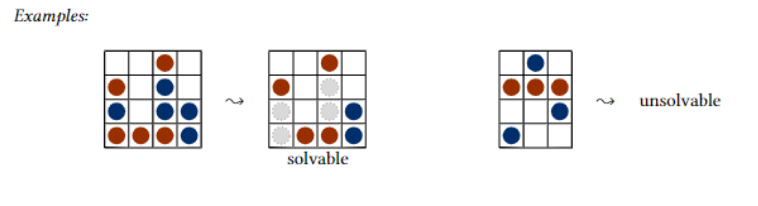
\includegraphics[width=1.3\linewidth]{image.png}
        \caption{From left to right: A solvable configuration, a solvable configuration, and an unsolvable configuration}
        \label{fig:Examples}
    \end{figure}
% \subsubsection*{Reduction idea}
% We can convert this problem to a \textbf{CNF} formula, such that each column is a clause and each row is a variable. This construction helps us have a variable for each row and we can further construct this by making two cells that are in the same row but have different colors to be a negation of the other.Cells that are colored in blue to be the negation of the ones colored in red.
% \subsubsection*{Redcution}
% Since we have defined how we can convert the problem to a \textbf{CNF}, we can form a \textbf{CNF} formula based on the table we have and we can therefore reduce it to \textbf{SAT} a well known \textbf{NPC} problem.
We consider a puzzle game where the board is a grid of \(n \times m\) squares, with each square containing a token that is either red or blue. The objective is to determine whether there exists a subset of tokens that can be removed such that:
\begin{enumerate}
    \item Every row has at least one token remaining.
    \item No column contains tokens of different colors.
\end{enumerate}

\section*{Proof of NP-Completeness}
\subsection*{Problem Definition}
Define the decision problem associated with the puzzle as follows:
\[
\text{PUZZLE-GAME} = \{(T, n, m) \mid \exists \text{ a valid subset of tokens } T \text{ in an } n \times m \text{ grid satisfying the conditions}\}
\]


\subsection*{NP Membership}
To show that PUZZLE-GAME is in NP, observe that any certificate or solution, which is a subset of tokens remaining on the board, can be verified in polynomial time. A verifier would need to check that:
\begin{itemize}
    \item Each row contains at least one token.
    \item No column contains both a red and a blue token simultaneously.
\end{itemize}

These steps can be done in a polynomial amount of time.

\subsection*{NP-Hardness}
To prove NP-hardness, we reduce the 3SAT problem (known to be NP-complete) to the PUZZLE-GAME problem. Consider an instance of 3SAT \(\phi\) with variables \(x_1, \dots, x_n\) and clauses \(C_1, \dots, C_m\).

\subsubsection*{Reduction from 3SAT to a PUZZLE-GAME}

To illustrate the reduction from a 3SAT problem to a satisfiability puzzle, consider the following construction:

\textbf{Grid Construction:}
\begin{itemize}
    \item Construct a grid with one row for each variable and one column for each clause in the 3SAT instance. Each cell in this grid, denoted as \(Cell[i, j]\), is capable of holding two tokens: one red and one blue.
    \item The red token in row \(i\) represents the positive literal \(x_i\) being part of clause \(C_j\), whereas the blue token represents the negated literal \(\overline{x_i}\) in the same clause.
    \item The overall time complexity of this will be $O(n\times m)$ where \(n\) is the number of variables or literals and \(m\) is the number of clauses. We get this as a result of constructing the $n \times m$ table from the instance of our 3SAT formula.
\end{itemize}

\textbf{Token Manipulation Rules:}
\begin{itemize}
    \item Each token in \(Cell[i, j]\) indicates the presence of a literal in clause \(C_j\). Removing a blue token implies setting the variable \(x_i\) to \texttt{false} for satisfying \(C_j\) and to \texttt{true} otherwise, and removing a red token means setting \(\overline{x_i}\) to \texttt{false} and \texttt{true} otherwise.
    \item This manipulation allows for a visual and interactive representation of variable assignments that satisfy the given 3SAT instance.
\end{itemize}

\textbf{Ensuring Satisfiability:}
\begin{itemize}
    \item To ensure a satisfying assignment, each row must retain at least one token. This corresponds to consistently assigning truth values across all clauses in which the variable appears.
    \item The configuration must also ensure that no column contains tokens of both colors, representing a scenario where a variable and its negation are both set to true, which is logically inconsistent.
\end{itemize}

This reduction effectively transforms the logical structure of a 3SAT problem into an instance of PUZZLE-GAME of tokens, where the challenge is to satisfy all clauses by appropriate token removals, thereby mapping directly to the satisfaction of the corresponding 3SAT instance. And since this reduction can be done in an amount of time that is a polynomial function of the input size of \(\phi\) we can say that 3SAT is karp reducible to PUZZLE-GAME and since PUZZLE-GAME is in NP and NP-Hard, we can say that PUZZLE-GAME is NP-Complete.

\subsection*{Conclusion}
Since we can reduce 3SAT to PUZZLE-GAME in polynomial time and verify solutions in polynomial time, PUZZLE-GAME is NP-complete.

\end{document}
